\chapter{Background}
\label{chapter:background}

The payoff function of these two types of derivatives can then simply be deduced as
\begin{equation}\label{callput}
\begin{split}
&\text{Payoff}_\text{call}(t)=(S(t)-K)^+;\\
&\text{Payoff}_\text{put}(t)=(K-S(t))^+,
\end{split}
\end{equation}
\noindent where $K$ is the strike price and $S(t)$ is the asset price at the time of exercise, $t$. These functions are represented in \autoref{fig:Payoff}.

\begin{figure}[H]
    \centering
      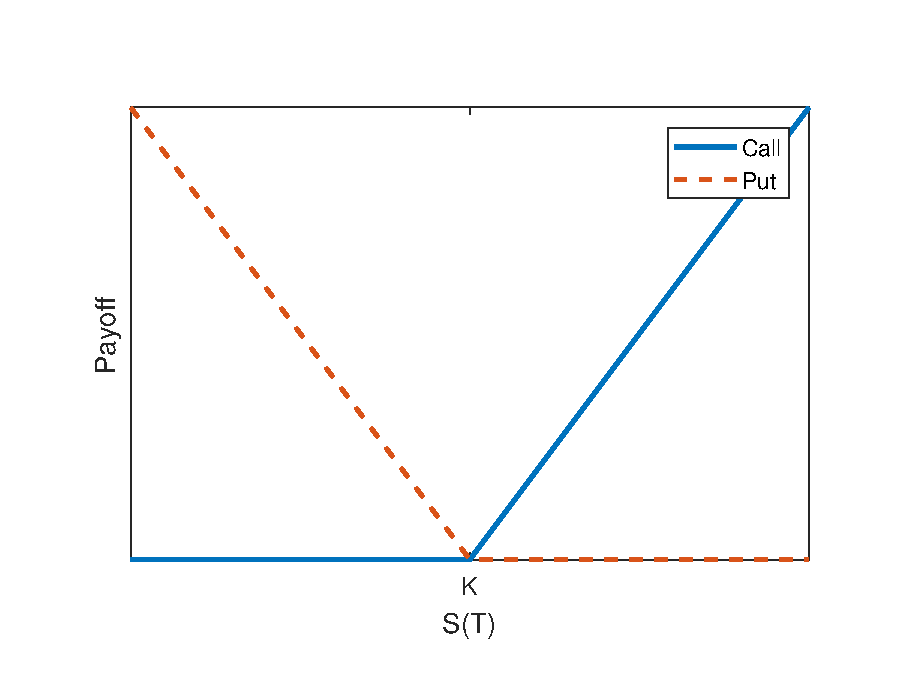
\includegraphics[width=.9\columnwidth]{Payoff.eps}
      \caption{Payoff functions of \textit{call} and \textit{put options}.}\label{fig:Payoff}
    \end{figure}
    
Due to their high importance, options have been studied in detail in the past.
Possibly the most important result in this field came from Fischer Black, Myron Scholes and Robert Merton, who developed a mathematical model to price European options~\cite{Scholes} - the famous Black-Scholes-Merton model - still in use in present days~\cite{Wilmott2}. The last two actually earned the 1997 Nobel prize in Economics for this development.

This model states that a European call or put option's price follows the partial differential equation (PDE)

\begin{equation}\label{BS2}
\pdv{V}{t}+\frac{1}{2}\sigma^2S^2\pdv{^2V}{S^2}+rS\pdv{V}{S}-rV=0,
\end{equation}

\noindent where $V$ is the price of the option, $S$ is the price of the underlying stock, $r$ is the risk-free interest rate and $\sigma$ is the stock price volatility.
Simply put, the volatility of a stock price is a measure of how uncertain the price movement is in the future. A high volatility will lead to great future fluctuations in the stock price.

This model assumes furthermore that stock prices follow a Geometric Brownian Motion (GBM), which can be defined as

\begin{equation}\label{BS}
dS(t)=rS(t)dt+\sigma S(t)dW(t),
\end{equation}
\noindent with $\{W(t),\ t>0\}$ defining a one-dimensional Brownian motion.

Because the stock price depends on a Brownian motion process, it follows that it is not differentiable. For this reason, it's impossible to exactly simulate such a process. An approximation is possible, however, using discrete jumps of length $\Delta t$ and using the Brownian motion property $W(t)\sim \sqrt{t}N(0,1)$~\cite{Mikosch}, with $N(0,1)$ being a normal distribution with 0 expected value and 1 variance.
We can then simply discretize eq. \eqref{BS} into
\begin{equation}
S(t+\Delta t)=S(t)+rS(t)\Delta t+\sqrt{\Delta t}\sigma S(t)N(0,1),
\end{equation}
\noindent where $\Delta t$ corresponds to a given time step. An example of this discretization is illustrated in \autoref{fig:GBM} with the realization of three sample paths.

\begin{figure}[H]
    \centering
      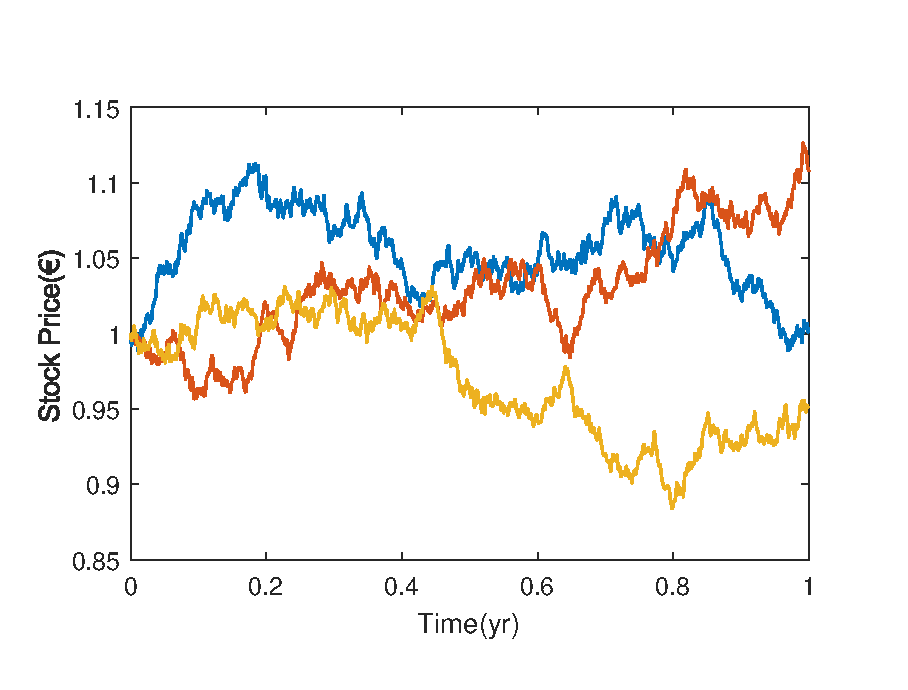
\includegraphics[width=0.9\columnwidth]{GBM.eps}
      \caption{Example of three GBM processes, using the parameters $r=\SI{0.06}{\per\year}$, $\sigma=0.05$, $S(0)=\SI{1}[\EUR]{}$ and time steps $\Delta t=10^{-3}\SI{}{\year}$.}\label{fig:GBM}
    \end{figure}
    
By simulating a large number of paths, some underlying tendencies might become apparent, which will prove useful in option pricing.

Pricing European options is fairly straightforward - we simply need to solve the PDE in eq. \eqref{BS2} in a similar fashion to the initial value problem for the diffusion
equation~\cite{Dilao}. American options, however, pose a much greater challenge.  Unlike European options, no analytic pricing model currently exists for this type of derivatives. Several numerical models have been proposed in the past in an attempt to solve this problem~\cite{Wilmott1,Hull}, such as the Longstaff-Schwartz algorithm~\citep{Longstaff}, which we shall approach in later sections of the present thesis.

\hl{!!!!!Put-call parity!!!!}
\hl{!!!!!American Puts=European Puts!!!!}



Insert your chapter material here...


%%%%%%%%%%%%%%%%%%%%%%%%%%%%%%%%%%%%%%%%%%%%%%%%%%%%%%%%%%%%%%%%%%%%%%%%
\section{Theoretical Overview}
\label{section:overview}

%!!!
\section{Put-Call parity}
\label{section:putcall parity}
%!!!

Some overview of the underlying theory about the topic...


%%%%%%%%%%%%%%%%%%%%%%%%%%%%%%%%%%%%%%%%%%%%%%%%%%%%%%%%%%%%%%%%%%%%%%%%
\section{Theoretical Model 1}
\label{section:theory1}

The research should be supported with a comprehensive list of references.
These should appear whenever necessary, in the limit, from the first to the last chapter.

A reference can be cited in any of the following ways:
%
\begin{itemize}
  \item Citation mode \#1 - \quad \cite{jameson:adjointns}
  \item Citation mode \#2 - \quad \citet{jameson:adjointns}
  \item Citation mode \#3 - \quad \citep{jameson:adjointns}
  \item Citation mode \#4 - \quad \citet*{jameson:adjointns}
  \item Citation mode \#5 - \quad \citep*{jameson:adjointns}
  \item Citation mode \#6 - \quad \citealt{jameson:adjointns}
  \item Citation mode \#7 - \quad \citealp{jameson:adjointns}
  \item Citation mode \#8 - \quad \citeauthor{jameson:adjointns}
  \item Citation mode \#9 - \quad \citeyear{jameson:adjointns}
  \item Citation mode \#10 - \quad \citeyearpar{jameson:adjointns}
\end{itemize}
%
Several citations can be made simultaneously as \citep{nocedal:opt,marta:ijcfd}. \\

This is often the default bibliography style adopted (numbers following the citation order), according to the options:\\
{\tt \textbackslash usepackage\{natbib\}} in file {\tt Thesis\_Preamble.tex},\\
{\tt \textbackslash bibliographystyle\{abbrvnat\}} in file {\tt Thesis.tex}.\\

Notice however that this style can be changed from numerical citation order to authors' last name with the options: \\
{\tt \textbackslash usepackage[numbers]\{natbib\}} in file {\tt Thesis\_Preamble.tex},\\
{\tt \textbackslash bibliographystyle\{abbrvunsrtnat\}} in file {\tt Thesis.tex}. \\

Multiple citations are compressed when using the {\tt sort\&compress} option when loading the {\tt natbib} package as {\tt \textbackslash usepackage[numbers,sort\&compress]\{natbib\}} in file {\tt Thesis\_Preamble.tex}, resulting in citations like \citep{marta:ijcfd1,marta:ijcfd2,marta:ijcfd3,marta:ijcfd4}.


%%%%%%%%%%%%%%%%%%%%%%%%%%%%%%%%%%%%%%%%%%%%%%%%%%%%%%%%%%%%%%%%%%%%%%%%
\section{Theoretical Model 2}
\label{section:theory2}

Other models...

